%! TEX root = **/010-main.tex
% vim: spell spelllang=en:

\subsection{Meta-learning algorithms}%
\label{sub:meta}

\subsubsection{Performance Majority Voting}

\begin{table}[H]
\centering
\caption{Majority voting results}
\begin{tabular}{lr}
\toprule
Method & Accuracy \\
\midrule
Na\"ive Bayes & 0.884 \\
K-NN & 0.857 \\
Decision Tree & 0.877 \\
\addlinespace[0.5em]
Majority voting & 0.914 \\
Majority voting (weighted)  & 0.914 \\
\bottomrule
\end{tabular}
\end{table}


With hard voting:
\sresults{ 375 &  33 \\ 20 & 172 }{ 0.9117 }

\noindent
With weighted voting (2 1 2):
\sresults{ 373 &  35 \\ 19 & 173 }{ 0.9100 }

There is no benefit to weighting the votes since all 3 methods offer very similar accuracy.
 
\pagebreak
\subsubsection{Bagging}

\begin{figure}[H]
\centering
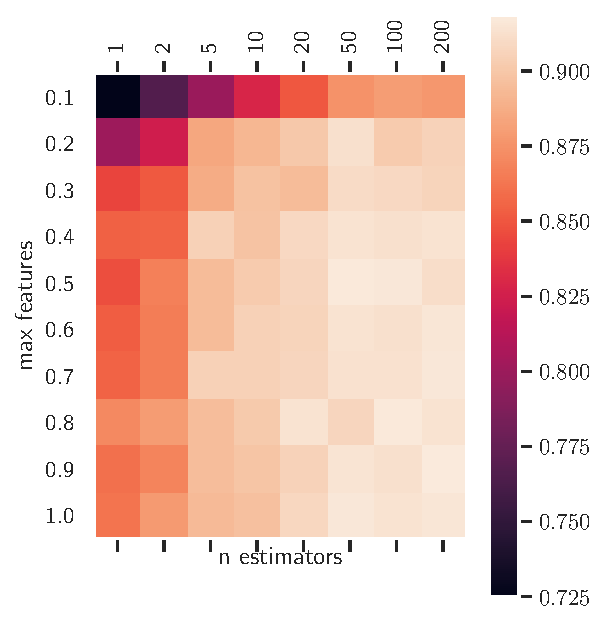
\includegraphics{bagging}
\caption{Bagging parameter search}%
\label{fig:bagging}
\end{figure}

The best results where obtained with: $\texttt{n\_est} = 200, \texttt{max\_features} = 0.9$. Nonetheless, as we
can see in \cref{fig:bagging} results with $\texttt{n\_est} \geq 50, \texttt{max\_features} \geq 0.3$ are pretty
similar.

\sresults{ 388 &  20 \\ 24  & 168 }{0.9267}

\begin{verbatim}
\end{verbatim}
 
\pagebreak
\subsubsection{RandomForest}

\begin{table}[H]
\centering
\caption{RandomForest best parameters}
\begin{tabular}{lr}
\toprule
Parameter & Value \\
\midrule
\texttt{bootstrap} & True \\
\texttt{max\_depth} & 150 \\
\texttt{max\_features} & 10 \\
\texttt{min\_samples\_leaf} & 5 \\
\texttt{min\_samples\_split} & 10 \\
\texttt{n\_estimators} & 100 \\
\bottomrule
\end{tabular}
\end{table}

\sresults{ 389 &  19 \\ 20 & 172 }{0.935}

\subsubsection{Adaboost}

The final algorithm we implemented is Ada boosting. The base implementation of this algorithms works with decision trees as it's classifier. This type of boosting basically consists on performing different executions of the classifier but changing the weights. The algorithm has two additional hyperparameters \texttt{n\_estimators} and \texttt{learning\_rate}.

After that we fined tuned the parameters and we found that the best combination is \texttt{n\_estimators} 0.4 and \texttt{learning\_rate} = 0.6

When executing Adaboost with the best parameters found we obtain the following results:

\fresults{ 383 &  25 \\ 21 & 171 }{0.923}{0.881}


% Performance  Majority  Voting,  Bagging, RandomForest  and  Adaboost.   Explain  parameters  selected  for  each  algorithm